 \chapter{RESULTS, DISCUSSIONS AND CONCLUSIONS} % Main chapter title
\label{ChapterResults} % For referencing the chapter elsewhere, use \ref{Chapter1} 
As every project starts with a goal to establish, a problem to solve and to make existing
projects better, they all lead to a result. These results helps us to determine whether the
approach taken, job done, analysis and research conducted was correct and up to the
mark or not. These results then help us to conclude what we have gained from all the
hassle of researching, developing and testing.

\section{Results \& Analysis}
The website, after several bug fizes and updates, feels very smooth and has good user experience as the client would want it. It is easily able to run both mobile phones and desktops. The following are the highlights of the website.
\\
1. The user experience is simple and elegant such that people of any age will easily be able to go through the website. 


2. The main page with the carousel is gesture friendly, it can be operated via gestures using mouse, hand gestures, touch pens..etc   -
\\
3. Mobile frindly even with a lot animations that have to load up. A lot of optimizations were done to the the gifs before exporting them so that it can easily be loaded on websites.
\\
4. The website is well adapted and tested to handle real time data, with instant changes in Google sheet data. The website automatically updates after a new refresh with the latest data from the google sheet data

\subsection{Images}

\begin{figure}[h]
	\begin{center}
		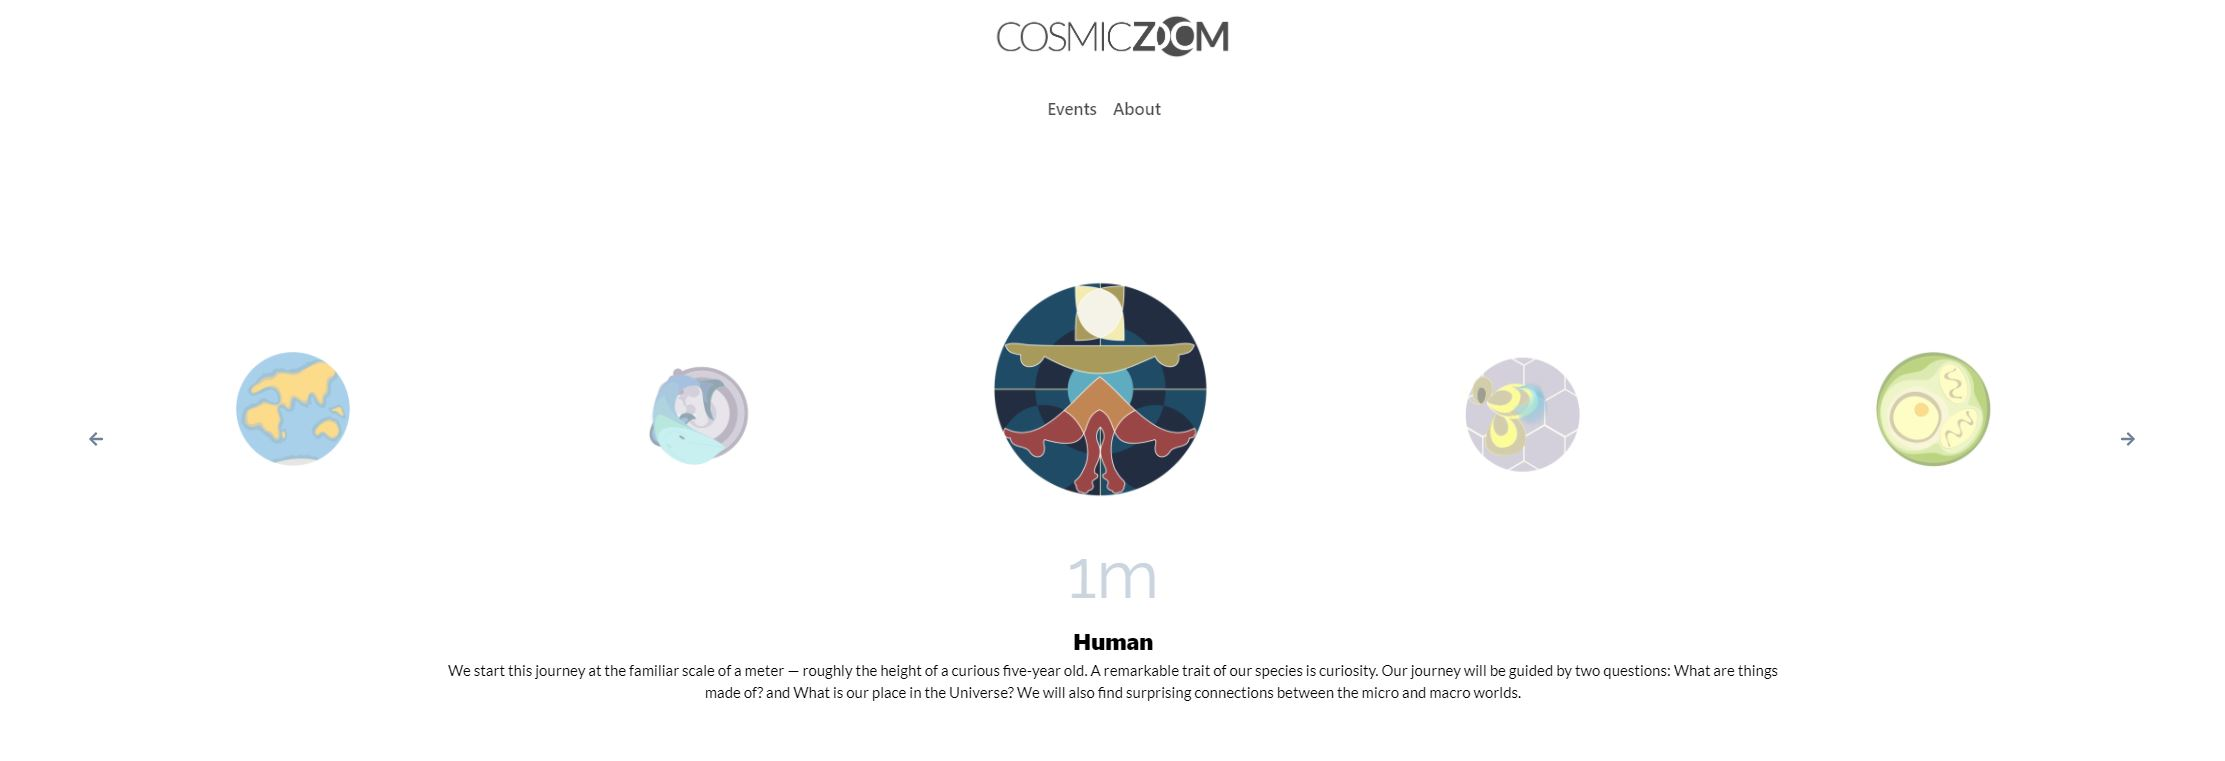
\includegraphics[scale=0.2]{Figures/web-1.JPG}
		\caption{Main page from a wide screen}
		\label{fig:rb}
	\end{center}
\end{figure}

\begin{figure}[h]
	\begin{center}
		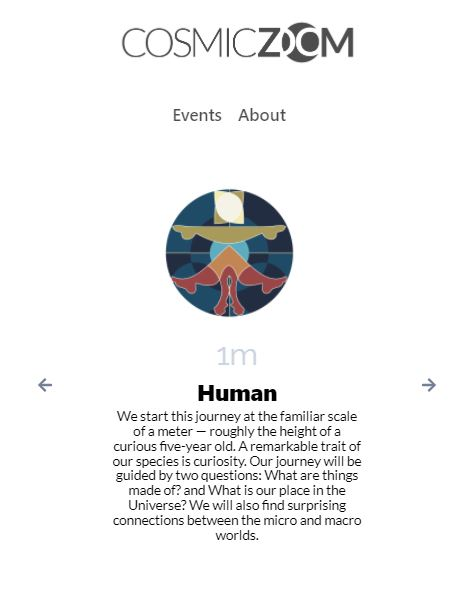
\includegraphics[scale=0.3]{Figures/mob-1.JPG}
		\caption{Main page from a mobile screen}
		\label{fig:rb}
	\end{center}
\end{figure}

\begin{figure}[h]
	\begin{center}
		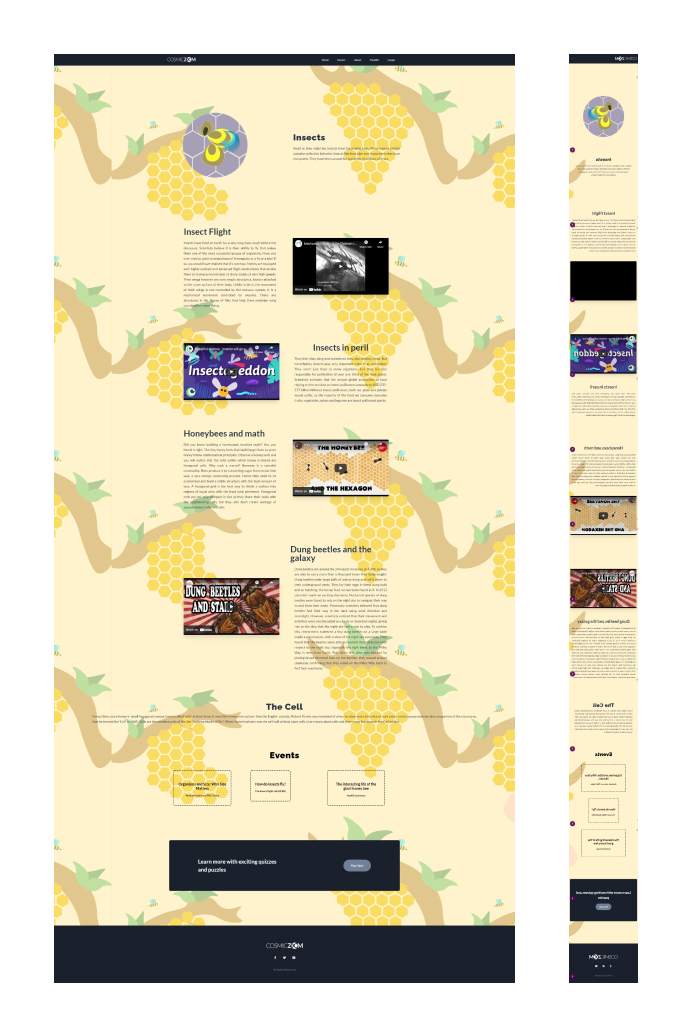
\includegraphics[scale=0.1]{Figures/mob-web.jpg}
		\caption{Insects scale page from a wide screen}
		\label{fig:rb}
	\end{center}
\end{figure}


\section{Comparative Study}
There are a lot of websites that are used to showcase various educational exhibits, some of the most notable one's are \href{https://firstladies.si.edu/gallery}{First Ladies of United States} and \href{https://www.npg.si.edu/}{National Portrait Gallery}. These were taken as an inspiration to design and develop the exhibition website, but make it more simple and user friendly. After the completion of the development process, here are a few
aspects that stand out from other dashboards:
\\
1. The application is made to look simple and is less straining to one's eye's when the all the focus is given only to the main content.
\\
2. The main page has a custom made carousel that is accessible very easily both on large and smaller screens.
\\
3. All the details come from a live google sheet that is continously being maintained for the latest and most accurate information and latest exhibits.


\section{Discussions}
This project opens up a lot of topics that can be discussed to educate common public, researchers, scholars, and students with various research and studies happening around them. It opens up the possibility to conduct online exhibitions with various other factors that can be included like quizzes, games, competitions..etc on  the internet 

\section{Conclusions}
The completeion of this project led to an online exhibition being called \href{https://cosmic-zoom.in/}{Cosmic-Zoom} held by \href{https://www.icts.res.in/}{ICTS(International Centre for Theoretical Sciences
)}, a centre of the Tata Institute of Fundamental Research which is a research institute which wanted to conduct an exhibition showcasing their research and scienctific discoveries in a storified manner through the website. 
This project led me to learn a lot of technoilogies and many Javascript libraries like react-router, styled-components, twin macro, framer motion and many many more. It also helped me look websites from a new perspective, of a designer as to how the user experience of a user can be increased and all components that are attached to this.


\section{Scope for Future Work}

1. Using a CDN to get the files and store in the user's cache is much better than loading it up at each reload
2. It is better to get data from a database rather than using Google Sheet API to get data from. The easy solution to this is to build an admin page that has access to the database, and has an editor like \href{https://quilljs.com/}{Quill.js} to be able to edit all the data, which will update on the website too.
3. More image optimization has to be done to let the image lazy-load only after all the other UI components and text have successfully loaded. This'll make it faster to browse the site from one page to the other very quickly.
 



	
	






